\documentclass[11pt]{article}
\usepackage[margin=1in]{geometry}
\usepackage{amsmath,amssymb,amsthm,mathtools}
\usepackage{booktabs,tabularx}
\usepackage{graphicx}
\usepackage[hidelinks]{hyperref}
\usepackage{xcolor}
\usepackage{enumitem}
\setlist{nosep,leftmargin=*}

\newtheorem{theorem}{Theorem}
\newtheorem{proposition}[theorem]{Proposition}
\newtheorem{lemma}[theorem]{Lemma}
\theoremstyle{definition}
\newtheorem{prediction}{Prediction}
\theoremstyle{remark}
\newtheorem{remark}[theorem]{Remark}

\newcommand{\E}{\mathbb{E}}
\newcommand{\Var}{\mathrm{Var}}
\newcommand{\Cov}{\mathrm{Cov}}
\newcommand{\I}{\mathcal{I}}
\newcommand{\src}[1]{\textsf{[#1]}}
\newcommand{\answer}[1]{\par\smallskip\noindent\fbox{\parbox{\dimexpr\linewidth-2\fboxsep-2\fboxrule}{\textbf{Answer.} #1}}\par\smallskip}

\title{When Can a Bandit Trust Correlation?\\[2pt]
\large Certified Pooling and Persistent Dynamics for Correlated Arms on the Web}
\author{Working long version, 12 October 2026 (revision 3)\\
\small Compiled from the \texttt{dependent\_mab} repository, to be condensed into a WWW 2027 submission}
\date{}

\begin{document}
\maketitle

\begin{abstract}
A short-video platform filling a daily trending slot faces arms that are correlated in two ways: videos watched by the same people tend to be liked by the same people, and a video's engagement today predicts its engagement for days. Platforms hold many graphs that seem to encode such structure, and graph bandits invite the learner to pool information along them. We ask when that trust is warranted.

We model every reward as $f_{i,t}=\mu_i+z_{i,t}$, with a \emph{mean channel} (long-run appeal $\mu$, restricted by a graph certificate) and a \emph{fluctuation channel} (persistent deviations $z$ with graph-correlated shocks), and test theory against data on three Web platforms (KuaiRec short video, Wikipedia attention, Open Bandit Dataset fashion recommendations) and controlled simulations. \textbf{Which correlation is real?} Collaborative graphs carry personal taste; social, profile and location graphs carry almost none. \textbf{How can a learner pool safely?} Certified pooling gains in proportion to the components its certificate can reject (rank correlation $-0.87$ across certificates on KuaiRec, $-0.81$ on the Open Bandit Dataset), uncertified pooling fails on informative graphs exactly as the misalignment theory predicts, and average gains come from shrinkage: real graphs beat their rewired nulls only under certification (8\% on KuaiRec). \textbf{What breaks when rewards persist?} We prove that certified pooling stays valid under persistent, correlated, restless sampling when its confidence sets come from an exact innovation regression, and that iid certificates fail under bursty exposure. Real Wikipedia attention sits in that failure regime (a week of consecutive views carries the information of 1.3--1.9 independent days, as long-run autocovariance fits predict); iid certificates are violated in 56--95\% of runs on worlds calibrated to it, and wrongly eliminate the best arm in up to 89\% of bursty runs, while innovation certificates stay valid even with estimated dynamics. Their cost is power: at Web persistence the anytime-valid widths are 10--25 times the information-limited width, so valid certificates rarely act. \textbf{How should a learner act on persistent fluctuations?} On a chronologically valid KuaiRec panel, persistence-aware policies halve regret against iid Thompson sampling, but the simplest persistence rule (the last observed value) captures the gain; a graph in the shock model helps only through a common factor.
\end{abstract}

\tableofcontents
\newpage

%=====================================================================
\section{Introduction}
%=====================================================================

\paragraph{A running example.} Every day a short-video platform shows ten videos in a trending slot. Two facts shape the decision. First, videos are related: those watched by the same audience tend to be enjoyed by the same audience, so evidence about one video is evidence about its neighbours. Second, engagement persists: a video's completion rate today predicts tomorrow's, and shocks such as a holiday or an outage hit many videos at once. The platform also holds many graphs that might encode the first fact (co-engagement, matrix-factorization neighbours, creator links, tags, a social network) and must decide which to use, if any.

\paragraph{Two ways to get it wrong.} A learner can \emph{trust correlation that is not there}: pooling along a graph whose neighbourhoods do not share appeal biases estimates, and in the worst case leads to linear regret. Or it can \emph{ignore that rewards persist}: confidence statements built for independent rewards are too narrow when consecutive observations of an item move together, so decisions that rely on them, such as dropping an item for good, go wrong. Both mistakes are easy to make on the Web, where graphs are by-products rather than designed priors and where exposure is bursty: the same items fill a slate day after day.

\paragraph{Model.} We write every reward as $f_{i,t}=\mu_i+z_{i,t}$. The \emph{mean channel} restricts long-run appeal $\mu$ with a graph certificate; the \emph{fluctuation channel} lets deviations $z$ follow an autoregression with graph-correlated shocks. Graphs are a tool for encoding correlation in either channel, not the object of study.

\paragraph{Four questions.} Table~\ref{tab:roadmap} lists the questions, the theory that makes each testable, and the answer the evidence gives. Each of Sections~\ref{sec:q1}--\ref{sec:q4} follows the same pattern: what theory says, what it predicts, what we find, and what it means.

\begin{table}[t]\centering\small
\begin{tabularx}{\linewidth}{p{2.7cm}p{4.2cm}X}
\toprule
Question & Theory that makes it testable & Answer from the evidence \\
\midrule
Q1. Which correlation is real? (\S\ref{sec:q1}) & Graph energy relative to gaps; smoothing changes the argmax; random graphs act as uniform shrinkage & Collaborative graphs carry taste; social, profile, location graphs barely do. Shocks: mostly a common factor; links add information only across communities with different rhythms. \\
Q2. How can a learner pool safely? (\S\ref{sec:q2}) & Certified pooling regret; gains only from components with width below gap & Gains track the rejectable share across certificates on two platforms. Uncertified pooling fails selectively. Real graphs beat rewired nulls only under certification. Practical certificates remain the bottleneck. \\
Q3. What breaks when rewards persist? (\S\ref{sec:q3}) & Innovation regression; certificates B1, B1$'$, B1$''$; failure result B2; long-run constants B3 & iid certificates fail under bursty exposure (85--95\% of toy runs, 56--95\% on Wikipedia-calibrated worlds), and real attention is in that regime. Innovation certificates stay valid, including with long-prefix estimated dynamics, but are too wide to act at Web persistence. \\
Q4. How should a learner act on persistent fluctuations? (\S\ref{sec:q4}) & Innovation lower bound; explore only uncertainty that persists & Persistence-aware policies halve regret against iid TS on a chronological panel; the last observed value captures the gain. Heavy exploration needs many observations per arm. The graph helps decisions through a common factor. \\
\bottomrule
\end{tabularx}
\caption{Roadmap: four questions, the theory behind each, and the answers.}\label{tab:roadmap}
\end{table}

\paragraph{Contributions.}
\begin{enumerate}
\item A two-channel model of correlated arms that contains iid bandits, static graph bandits and restless autoregressive bandits as special cases, and separates what a graph can encode (\S\ref{sec:model}).
\item \textbf{Theory bridging the channels} (\S\ref{sec:q3}, proofs in Appendix~\ref{app:proofs}): certified pooling is valid under persistent, correlated, restless sampling when built on an exact innovation regression (B1); scalar certificates for independent shocks (B1$'$) and, by iterated nuisance plug-in, for correlated shocks (B1$''$); a quantitative failure result for iid certificates (B2); long-run substitution of the mean-channel constants and the general slate-contrast formula (B3).
\item \textbf{Predictions tested against data.} Each theoretical statement yields a prediction that we test, including on real or real-calibrated dynamics: certified gains track rejectable components on two platforms (\S\ref{sec:q2}); B2's variance inflation appears in real Web attention and predicts certificate failures (\S\ref{sec:q3}); B3's long-run constants predict held-out inflation (\S\ref{sec:q3}).
\item \textbf{Measurements on three Web platforms} (KuaiRec short video, under a chronologically valid protocol for the dynamic experiments; Wikipedia attention; Open Bandit Dataset click rates) with standard non-stationary baselines, and a controlled 100-arm spatiotemporal benchmark.
\end{enumerate}

\paragraph{What changed from revision 2.} Revision 2 (9 October) relied on a KuaiRec daily panel whose item graph used future interactions and on Wikipedia panels selected with later data. Revision 3 re-runs the KuaiRec daily experiment chronologically with standard baselines, expands certified-pooling experiments to 360 instances, adds the Open Bandit Dataset, tests certificates with estimated and misspecified dynamics and on worlds calibrated to real attention, measures B2's inflation on real data, and checks B3 exactly. Several revision-2 claims change: see \S\ref{sec:changes}.

\paragraph{Provenance.} Results proved in companion manuscripts in the repository are labelled \src{A} (graph alignment and certified pooling), \src{S} (spatiotemporal filtering and confidence), \src{P} (predictive and AR bandits) and \src{N} (a repository note on the selection index). Results first stated here are labelled \src{New}.

%=====================================================================
\section{Setting: two channels of correlation}\label{sec:model}
%=====================================================================

There are $N$ arms. In round $t$ the learner pulls one arm, or a slate $S_t$ of $k$ arms, and observes
\begin{equation}\label{eq:model}
Y_t=\mu_{a_t}+z_{a_t,t}+\xi_t,\qquad z_t=\sum_{r=1}^{p}A_r z_{t-r}+\eta_t,\qquad \eta_t\sim N(0,Q_G),\qquad \xi_t\sim N(0,r).
\end{equation}
Every arm evolves every round (restless); only pulled arms are observed.

\paragraph{Mean channel.} Long-run means $\mu\in[0,1]^N$ are unknown. A graph supplies either a partition $\{C_c\}$ with certified diameters $\varepsilon_c\ge\max_{i\in C_c}\mu_i-\min_{i\in C_c}\mu_i$, or an energy certificate $\mu_c^\top L_c\mu_c\le S_c^2$, which implies diameters through effective resistance \src{A}.

\paragraph{Fluctuation channel.} Deviations persist through $A_r$ and are correlated across arms through $Q_G$, which can be shrunk toward a graph kernel. A shock common to all arms (a holiday) and a shock common to a community (a league's game day) are both correlation; only the second is something a graph can tell apart from a common factor.

\paragraph{Regret.} \emph{Mean regret} $\sum_t(\mu^\star-\mu_{a_t})$ measures learning of persistent appeal. \emph{Dynamic regret} $\sum_t(\max_i f_{i,t}-f_{a_t,t})$ measures tracking of current rewards against an oracle that sees every arm's current value. With slates, both are summed over the slate against the oracle's top $k$.

\paragraph{Special cases.} iid bandits: $A_r=0$, $Q_G$ diagonal, no certificate. Static graph bandits: $A_r=0$ with a mean certificate. Restless AR bandits: no mean certificate. Spectral bandits regularize the mean channel without certifying it.

%=====================================================================
\section{Q1. Which correlation is real?}\label{sec:q1}
%=====================================================================

\subsection{What theory says}

For the mean channel, a graph helps only if long-run appeal is smooth on it relative to the gaps that matter. Two facts sharpen this \src{A,N}. Smoothing on a complete graph shrinks all arms toward a common value and preserves every ranking; smoothing on an informative graph pulls an arm toward its neighbourhood's level, which can change the best arm (the misalignment example: $\mu=(1,0.9,0)$ with arms 1 and 3 linked makes arm 2 best after smoothing). So a graph can be \emph{smoother than chance} and still \emph{unsafe to smooth}. For the fluctuation channel, a graph helps only if shocks are correlated along its edges beyond what a single common factor explains.

\begin{prediction}\label{pred:q1}
(a) Graphs built from collaborative signals align with personal taste more than graphs built from profiles or content. (b) Fixed smoothing on informative graphs changes users' best items more than smoothing on rewired graphs. (c) A graph improves the shock model only if shocks are community-specific.
\end{prediction}

\subsection{Evidence: the mean channel on KuaiRec}

KuaiRec contains a 1,411 user $\times$ 3,327 video matrix that is 99.6\% observed. A larger sparse matrix (7,176 $\times$ 10,728) shares no (user, video) pair with it, so every graph is built leakage-free: user-side signals use only non-evaluation videos and video-side signals only non-evaluation users. We build sixteen graphs (Appendix~\ref{app:data}) and compare each with a degree-preserving rewiring. Table~\ref{tab:align} and Figure~\ref{fig:align} report three measures: a smoothness quotient (Laplacians scaled so a random graph scores about 1), the correlation of neighbours' personal taste after removing each user's activity and each video's popularity, and the cost to each user's best choice of smoothing true means with $(I+10L)^{-1}$.

\begin{table}[t]\centering\small
\resizebox{\linewidth}{!}{%
\begin{tabular}{lcccc}
\toprule
Graph & Side & Quotient (real / rewired) & Personal-taste corr. (real / random) & Choice cost, $\lambda{=}10$ (real / rewired) \\
\midrule
I-mf (factorization) & item & 0.756 / 0.961 & \textbf{0.046} / 0.002 & 0.117 / 0.019 \\
I-coeng (co-engagement) & item & 1.098 / 1.302 & \textbf{0.034} / 0.002 & 0.131 / 0.037 \\
I-cat / I-tag (content) & item & 0.908 / 0.985, 0.943 / 1.010 & 0.010 / 0.002 & 0.099 / 0.079, 0.100 / 0.054 \\
I-coauthor (same creator) & item & 0.805 / 1.006 & 0.004 / 0.002 & 0.040 / 0.184 \\
U-coeng (co-engagement) & user & \textbf{0.649} / 0.791 & \textbf{0.020} / 0.000 & 0.284 / 0.291 \\
U-coauthor, U-coeng-idf & user & 0.761 / 0.871, 0.748 / 0.860 & 0.018 / 0.000 & 0.296 / 0.294 \\
U-mf (factorization) & user & 0.850 / 0.907 & 0.016 / 0.001 & 0.300 / 0.298 \\
U-cotag, U-cotime & user & 0.842 / 0.884, 0.931 / 0.947 & 0.004, 0.003 & 0.299 / 0.297, 0.315 / 0.304 \\
U-geo, U-feat, U-demo & user & 0.946, 0.972, 0.988 & 0.007, 0.006, 0.002 & 0.350, 0.305, 0.328 \\
U-soc (social; 47 edges) & user & not comparable & 0.035 per edge & -- \\
\bottomrule
\end{tabular}}
\caption{KuaiRec: which graphs encode correlated appeal (reward = capped watch ratio, $k=10$).}\label{tab:align}
\end{table}

\begin{figure}[t]\centering
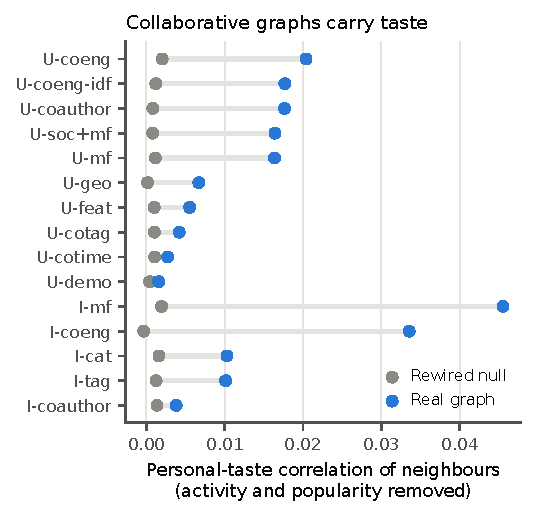
\includegraphics[width=0.5\linewidth]{../figures/f1_alignment.pdf}
\caption{Personal-taste correlation of graph neighbours, real graph against its rewiring.}\label{fig:align}
\end{figure}

\paragraph{Findings.}
\begin{itemize}
\item \emph{Collaborative graphs carry taste} (Prediction~\ref{pred:q1}a). Factorization and co-engagement neighbours agree on personal taste at 17--23 times the random-pair level; tag, category and creator graphs mostly group videos of similar popularity. Among user graphs, co-engagement is best; profile, location and demographic graphs are close to random. The social graph covers only 80 of 1,411 users. Rankings are stable across $k\in\{5,10,20\}$ and under a binary like-based reward (rank correlation 0.80).
\item \emph{Smoother than chance is not safe to smooth} (Prediction~\ref{pred:q1}b). On item graphs, fixed smoothing costs more of a user's best-choice value on the real graph than on its rewiring (I-mf at $\lambda=10$: 0.117 against 0.019). The rewiring acts like uniform shrinkage; the real graph pulls videos toward their community, which reorders the top. The exception (I-coauthor) makes small cliques of near-identical videos.
\end{itemize}

\subsection{Evidence: the fluctuation channel on three panels}

Table~\ref{tab:shocks} compares shock correlation along graph edges, along rewired edges and across all pairs, and the held-out likelihood of the innovation covariance under each graph target, on three daily panels: KuaiRec (253 videos, 63 days), Wikipedia programming-language articles (150 articles, 2022--2025) and Wikipedia articles from six communities (25 each). The six-community panel was designed after the first two returned a null, to test Prediction~\ref{pred:q1}c directly. The Wikipedia panels were selected with 2022--2025 data and use a 2026 hyperlink snapshot, so their graph results are retrospective; on KuaiRec, a chronological re-run with a prefix-only graph (\S\ref{sec:q4}) gives the same null.

\begin{table}[t]\centering\small
\resizebox{\linewidth}{!}{%
\begin{tabular}{lcccc}
\toprule
Panel & Graph & Shock corr.: edges / rewired / all & Within / across communities & Held-out log-lik per day: graph / rewired / common factor \\
\midrule
KuaiRec daily & co-engagement & 0.071 / 0.068 / 0.042 & -- & $-323.0$ / $-323.3$ / $\mathbf{-305.7}$ \\
Wikipedia, one domain & hyperlinks & 0.256 / 0.250 / 0.218 & -- & 52.88 / 52.85 / \textbf{53.76} \\
Wikipedia, six domains & hyperlinks & \textbf{0.273} / 0.051 / 0.051 & 0.320 / 0.000 & \textbf{22.16} / 21.67 / 21.92 \\
\bottomrule
\end{tabular}}
\caption{Do graphs carry correlated shocks? Held-out log-likelihood scores AR residuals under each innovation-covariance target fitted on the preceding window, averaged over three origins. Domain blocks score 22.13 on the six-domain panel.}\label{tab:shocks}
\end{table}

\paragraph{Findings.}
\begin{itemize}
\item On KuaiRec and on single-domain Wikipedia, shocks are correlated, but through a platform- or domain-wide factor: graph edges are no more correlated than rewired edges, and a common-factor covariance fits held-out shocks best.
\item With six communities, the picture reverses (Prediction~\ref{pred:q1}c). Shocks correlate at 0.32 within a community and 0.00 across; 84\% of hyperlinks stay within a community, so hyperlinked pairs correlate at 0.273 against 0.051 for rewired pairs, and hyperlinks give the best held-out fit, matching an oracle community-block graph.
\end{itemize}

\answer{For long-run appeal, trust collaborative graphs (factorization, co-engagement) and treat profile, location, social and content graphs as popularity signals. Even a good graph is not safe to smooth with a fixed strength. For fluctuations, a common factor captures most shared shocks; a graph adds information only when the arms span communities with different rhythms (a retrospective finding that awaits a chronological check).}

%=====================================================================
\section{Q2. How can a learner pool safely?}\label{sec:q2}
%=====================================================================

\subsection{What theory says}

\paragraph{Certified pooling \src{A}.} SP-UCB keeps an arm upper bound $u_i=\bar Y_i+b(n_i)$, $b(n)=\sigma\sqrt{2\ell/n}$, and a pooled component bound, selects the component maximizing $U_c=\min\{\max_{i\in C_c}u_i,\ \hat p_c+b(N_c)+\varepsilon_c\}$ and pulls its best arm. SP-KLUCB replaces both radii with Bernoulli KL bounds at the same fixed level.

\begin{theorem}[Alignment-sensitive regret \src{A}]\label{thm:spucb}
With valid certificates, with probability at least $1-\delta$,
$\mathcal R_T\le\sum_{c\in\mathcal O}A_c+\sum_{c\notin\mathcal O}\min\{A_c,H_c\}$, where $A_c=\sum_{i\in C_c:\Delta_i>0}(\Delta_i+8\sigma^2\ell/\Delta_i)$ is the cost of exploring the component arm by arm and $H_c=(\Gamma_c+\varepsilon_c)(1+8\sigma^2\ell/(\Gamma_c-\varepsilon_c)^2)$ is the cost of rejecting it as a whole, finite only when its width $\varepsilon_c$ is below its gap $\Gamma_c$.
\end{theorem}

Graph geometry, not diameter, sets the value of a certificate: a path and a clique with identical diameters and energy budgets differ in information cost by a factor growing with the component size, and the cost of loosening a certificate grows with the resistance radius \src{A}. These geometry results are tested in simulation only \src{A}.

\begin{prediction}\label{pred:q2}
(a) Certified pooling gains only through components whose width is below their gap: gains should rise with the share of such \emph{rejectable} components, across certificates and platforms. (b) Pooling with zero width (no certificate) fails when the optimal arm's component has a lower average than another component. (c) Average gains come mostly from shrinkage, so rewired graphs should do about as well on average; a real graph can help only through the components its certificate makes rejectable.
\end{prediction}

\subsection{Evidence on KuaiRec}

\paragraph{Design (Setting A).} For each test user, 300 videos are sampled and each item graph is rebuilt on them; SP-KLUCB uses a 20-component spectral partition; rewards are Bernoulli with the user's true means; $T=20{,}000$; common random numbers across policies. Revision 3 uses 120 held-out users $\times$ 3 video subsets (360 instances; the first 60 reproduce revision 2's table exactly). Certificates: oracle widths (true within-component range), energy (from the graph), population-calibrated (a quantile over tuning users), per-user calibrated (tuning users of similar level, after a paid warm-up), and none. Ratios are to KL-UCB at the same fixed level; we report the ratio of mean regrets with a user bootstrap and the mean of per-instance ratios, which weight users differently.

\begin{table}[t]\centering\small
\resizebox{\linewidth}{!}{%
\begin{tabular}{lccccc}
\toprule
SP-KLUCB certificate (I-mf) & Ratio of means [95\% CI] & Mean of ratios / 90th pct. & Components valid & Suboptimal rejectable & Mean width \\
\midrule
Oracle (true within-component range) & \textbf{0.64} [0.61, 0.67] & 0.80 / 1.04 & 100\% & 59\% & 0.38 \\
Per-user calibrated, 75th percentile & 0.82 & 0.90 / 1.04 & 74\% & -- & 0.42 \\
Population calibrated, 50th percentile & 0.70 [0.66, 0.73] & 0.83 / 1.04 & 47\% & 62\% & 0.30 \\
Per-user calibrated, 90th percentile & 0.95 & 0.97 / 1.04 & 89\% & -- & 0.63 \\
Population calibrated, 90th percentile & 0.99 [0.98, 0.99] & 0.99 / 1.04 & 90\% & 15\% & 0.71 \\
Energy (from the graph) & 0.96 [0.95, 0.97] & 0.98 / 1.04 & 100\% & 21\% & 0.80 \\
None (zero width) & 0.37 [0.35, 0.40] & 0.62 / 1.08 & 0\% & 95\% & 0 \\
\bottomrule
\end{tabular}}
\caption{The certificate gap (Setting A v2, 360 instances, KL bounds). All certified variants stay at or below 1.04$\times$ KL-UCB at the 90th percentile. In absolute terms Thompson sampling beats every fixed-level KL policy (oracle SP-KLUCB is 1.46$\times$ TS on I-mf), so claims are within the KL family.}\label{tab:certgap}
\end{table}

\begin{figure}[t]\centering
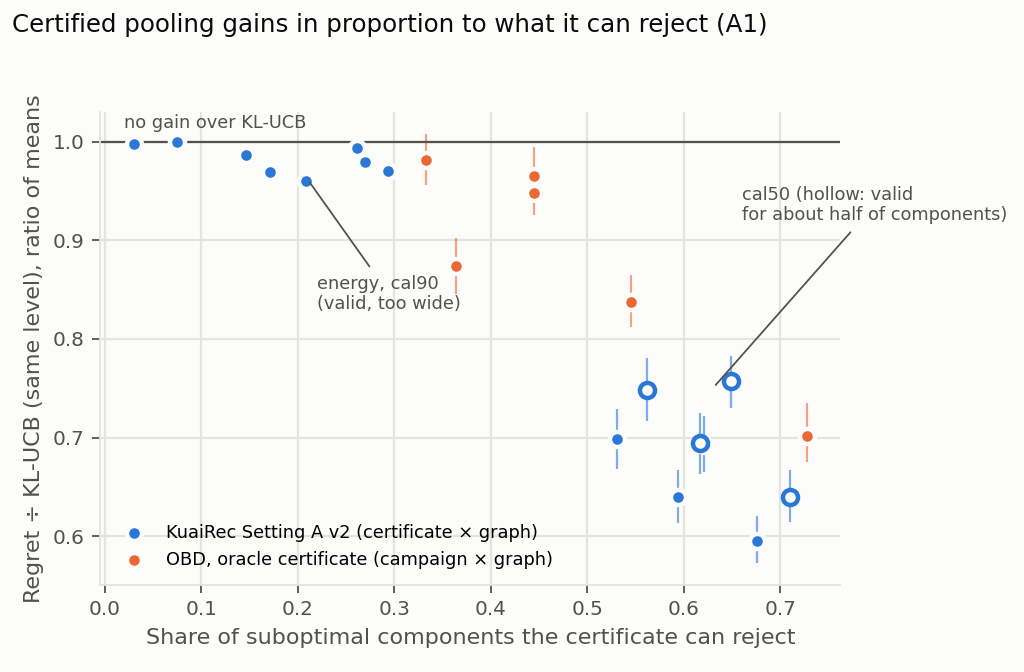
\includegraphics[width=0.85\linewidth]{../figures/r1_dose_response.png}
\caption{Certified pooling gains in proportion to the share of suboptimal components its certificate can reject. Points: certificate $\times$ graph on KuaiRec (360 instances each) and campaign $\times$ grouping on the Open Bandit Dataset (oracle certificate, 20 seeds each); hollow points are certificates valid for under 85\% of components.}\label{fig:dose}
\end{figure}

\paragraph{Findings.}
\begin{itemize}
\item \emph{Gains follow the theorem across certificates} (Prediction~\ref{pred:q2}a; Figure~\ref{fig:dose}). Across the 16 certificate $\times$ graph cells, the regret ratio falls with the rejectable share (Spearman $-0.87$). Valid but wide certificates (energy, 90th-percentile calibration) reject 15--29\% of suboptimal components and gain 1--4\%; the oracle rejects 59--68\% and gains 30--40\% (ratio of means). Within one certificate, the per-instance link is weaker than revision 2 reported with UCB1 and 60 users (Spearman $-0.48$ then; $-0.09$ now with KL bounds over 1,440 oracle instances): the median ratio falls from 0.91 to 0.68 as the rejectable share rises to 70--85\%, then rebounds to 0.95 above 85\%. Rejectability predicts \emph{which certificate} helps better than \emph{which instance} it helps.
\item \emph{Uncertified pooling fails selectively} (Prediction~\ref{pred:q2}b). Zero-width pooling is best on average (0.37 ratio of means) but carries the tail: on I-tag its 90th percentile is 1.74$\times$ KL-UCB, and spectral Thompson sampling on I-coeng regrets 1.54$\times$ TS on average with 27\% of users above 2$\times$. In revision 2's per-instance analysis, failures occurred when the optimal arm's component was not the top component by average (90th percentile 1.19$\times$ UCB1, against 0.37$\times$ when it was), on informative graphs (38\% of users on the creator graph) and never on the rewired graph. In Setting B (300 users arriving at random), user pooling without a certificate is 39\% worse than none.
\item \emph{Average gains are shrinkage; structure helps only under certification} (Prediction~\ref{pred:q2}c; Figure~\ref{fig:rewired}). Paired on 360 instances, oracle-certified SP-KLUCB regrets $0.916\times$ on the real I-mf graph against its rewiring [0.905, 0.926]: the real graph makes more components rejectable (59\% against 53\%). Uncertified pooling ($1.03$ [0.96, 1.10]) and spectral Thompson sampling ($1.00$ [0.96, 1.05]) are indistinguishable from the rewired null. Graph-free shrinkage (Gaussian Thompson sampling on the complete graph, $\lambda=10$) is the best average policy (0.69$\times$ TS). In Setting B, shrinking toward the population mean cuts regret 27\% and no user graph beats it.
\end{itemize}

\subsection{Replication on the Open Bandit Dataset}

\paragraph{Design.} The Open Bandit Dataset logs ZOZOTOWN fashion recommendations under a uniform-random policy (7 days; 1.37M impressions over 80 items in the All campaign, 0.86M over 46 items in Women; click rate 0.35--0.48\%). Item click rates are learnable: the between-item spread is 3.1--3.5 times its sampling error, and days 1--3 predict days 4--7 with correlation 0.49--0.71. We treat days 4--7 click rates as true means and build components from days 1--3 only: released item-attribute groups, audience-response clusters (k-means on click profiles over user segments), and shuffled attribute labels as the null. Policies serve blocks of 100 impressions per decision for 2M impressions; 20 seeds. This is semi-synthetic evidence: real parameters, simulated clicks.

\begin{table}[t]\centering\small
\begin{tabular}{lcccccc}
\toprule
& \multicolumn{3}{c}{All} & \multicolumn{3}{c}{Women} \\
Policy (regret $\div$ KL-UCB, fixed level) & attr & audience & shuffled & attr & audience & shuffled \\
\midrule
SP-KLUCB, oracle certificate & 0.84 & \textbf{0.70} & 0.87 & 0.98 & 0.97 & 0.95 \\
SP-KLUCB, prefix-range certificate & 0.86 & 0.78 & 0.87 & 1.01 & 0.81 & 1.01 \\
SP-KLUCB, no certificate & 0.66 & 0.60$^\dagger$ & 0.41 & 1.14 & 0.88 & 0.34 \\
Suboptimal components rejectable (oracle) & 55\% & 73\% & 36\% & 33\% & 44\% & 44\% \\
\midrule
Empirical-Bayes TS (graph-free) & \multicolumn{3}{c}{\textbf{0.21}} & \multicolumn{3}{c}{\textbf{0.29}} \\
Beta TS & \multicolumn{3}{c}{0.35} & \multicolumn{3}{c}{0.39} \\
\bottomrule
\end{tabular}
\caption{Open Bandit Dataset, regret at 2M impressions relative to KL-UCB at the same fixed level, paired by seed. $^\dagger$Never finds the best item; regret grows linearly (959, 1,442, 2,353 clicks lost at 0.5M, 1M, 2M impressions).}\label{tab:obd}
\end{table}

\paragraph{Findings.} The three predictions replicate (Table~\ref{tab:obd}). The oracle gain tracks the rejectable share (Spearman $-0.81$ over the six cells; largest gain 0.70 where 73\% of components are rejectable, 2--5\% where a third are). Uncertified pooling locks onto the wrong group on audience clusters and is 3.3$\times$ worse on real attribute groups than on shuffled ones in Women, while shuffled groups act as harmless global shrinkage. Graph-free empirical-Bayes shrinkage is best by a wide margin. The prefix-range certificate covers the true within-component range in only 25--70\% of components, because click rates drift between the halves; the empirically best item is the true best with posterior probability only 0.32--0.73.

\begin{figure}[t]\centering
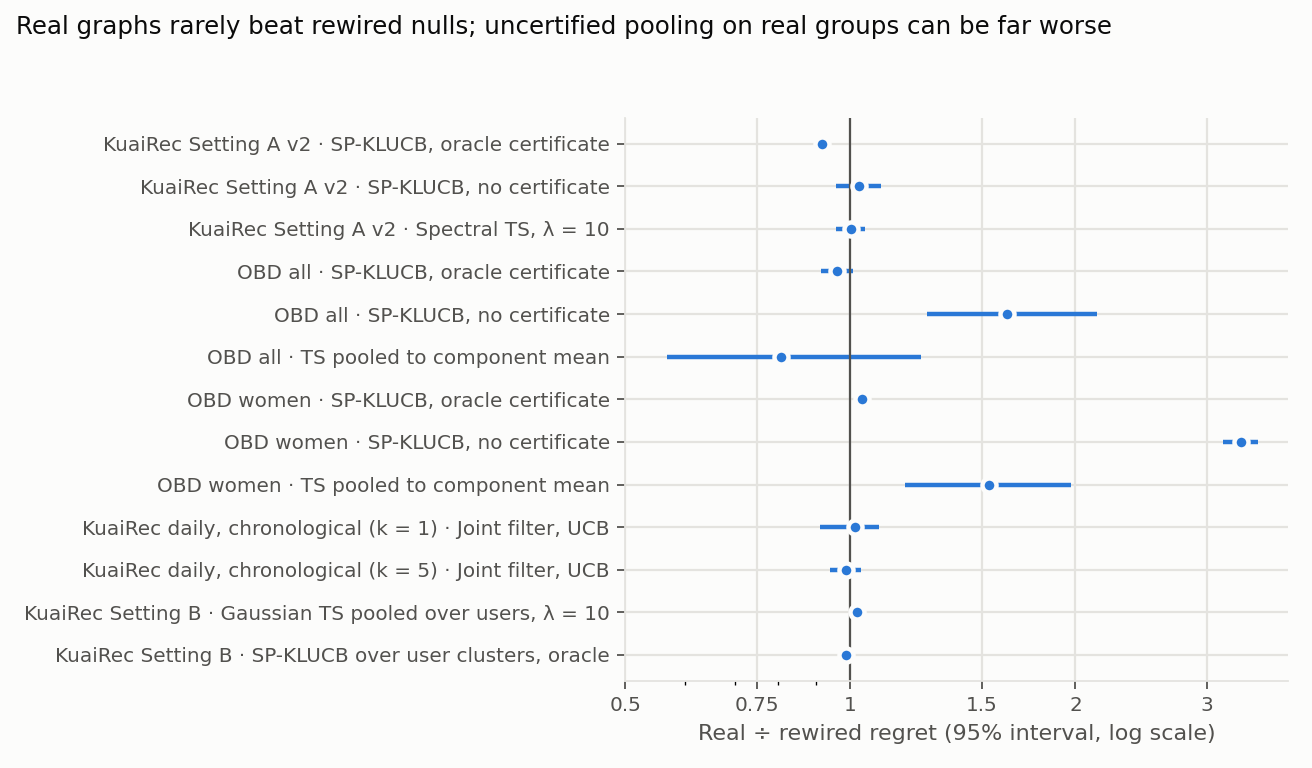
\includegraphics[width=0.9\linewidth]{../figures/r2_real_vs_rewired.png}
\caption{Paired regret ratios, real graph over its rewiring (shuffled groups on the Open Bandit Dataset), with 95\% bootstrap intervals over users, seeds or units.}\label{fig:rewired}
\end{figure}

\answer{Pool only with a certificate, and expect gains in proportion to the components the certificate can reject; this holds across certificates on two platforms. Uncertified pooling looks good on average but fails selectively on informative graphs. Graph structure adds value over a random graph only through certified rejection; average gains are shrinkage, which a graph-free empirical-Bayes prior delivers best. The open problem is a certificate that is both valid and narrow; level-matched calibration closes about half of the gap.}

%=====================================================================
\section{Q3. What breaks when rewards persist?}\label{sec:q3}
%=====================================================================

\subsection{What theory says}

Certified pooling relies on confidence bounds. With persistent, restless rewards, consecutive observations of an arm are correlated, and an arm's current value is partly predictable from the past. The \emph{innovation regression} of \src{S} removes the predictable part exactly.

\begin{theorem}[Predictable innovation experiments \src{S}]\label{thm:innov}
Conditional on a candidate mean $\mu$, a Kalman recursion that does not depend on $\mu$ gives, for the chosen arm, $R_t=u_t^\top\mu+\epsilon_t$ with predictable $u_t$ and $\epsilon_t\mid\mathcal H_t\sim N(0,1)$. With $J_T=H+\sum_tu_tu_t^\top$, $\hat\mu_T=J_T^{-1}\sum_tu_tR_t$ and a self-normalized width $\beta_T$, $|v^\top(\hat\mu_T-\mu)|\le\beta_T\|v\|_{J_T^{-1}}$ for all $T$ and all $v$ with probability at least $1-\delta$.
\end{theorem}

Building SP-UCB's bounds from this regression gives the following results (statements here, proofs in Appendix~\ref{app:proofs}).

\begin{theorem}[B1: validity and regret \src{New}]\label{thm:b1}
With valid certificates and correctly specified dynamics, the innovation-based arm and component bounds hold at every round with probability at least $1-\delta$, under any adaptive restless schedule. If each pull adds information at least $\iota$ to the relevant contrast, Theorem~\ref{thm:spucb} holds with $8\sigma^2\ell$ replaced by $4\beta_T^2/\iota$; for independent AR(1) arms, $\iota\ge(1-\varphi)^2/(V+r)$.
\end{theorem}

B1 is valid but wide: its width carries an $N$-dimensional log-determinant (about 12 standard errors with 20 arms and $T=20{,}000$, against about 5.5 for a per-arm bound).

\begin{proposition}[B1$'$: independent shocks \src{New}]\label{prop:b1p}
If $Q_G$ is diagonal, the innovation information is diagonal and every arm and component statistic is a scalar martingale; one-dimensional mixture bounds with a union over the $N+M$ statistics are valid and about as narrow as iid bounds.
\end{proposition}

\begin{proposition}[B1$''$: correlated shocks \src{New}]\label{prop:b1pp}
With correlated shocks, other arms' means enter each arm's regression as bounded nuisances $\sum_{j\ne i}G_{ij}(\mu_j-m_j)$, $G=J-\alpha I$. On the event that all scalar mixture bounds hold, plugging in intervals that contain the truth yields intervals that contain the truth, so iterating from $[0,1]$ is valid. Writing $\mu_i=\theta_c+d_i$ with $|d_i|\le\varepsilon_c/2$ gives a valid pooled component bound; with independent shocks it reduces to SP-UCB's.
\end{proposition}

\begin{proposition}[B2: iid certificates under persistence \src{New}]\label{prop:b2}
If an AR(1) arm with persistence $\varphi$ is pulled in blocks of $b$ consecutive rounds, the sample mean's standard deviation is inflated by $\sqrt{f(b,\varphi)}$, $f(b,\varphi)=\frac{1+\varphi}{1-\varphi}-\frac{2\varphi(1-\varphi^b)}{b(1-\varphi)^2}$, so the iid radius $\sqrt{2\sigma^2\ell/n}$ has per-check miscoverage $2\Phi(-\sqrt{2\ell}/\sqrt{f(b,\varphi)})$. For a general stationary process, $f(b)=1+2\sum_{h<b}(1-h/b)\rho(h)$ with the full autocorrelation function $\rho$.
\end{proposition}

\begin{proposition}[B3: long-run constants and slates \src{New}]\label{prop:b3}
(1) Under long runs or full slates with common AR coefficients, all mean-channel constants of \src{A} hold with $\sigma^2$ replaced by the long-run variance $q/c^2$, $c=1-\sum_ra_r$ (for AR(1), $V(1+\varphi)/(1-\varphi)$). (2) Two arms observed $n$ times each have long-run contrast variance $(\Omega_{ii}+\Omega_{jj}-2\Omega_{ij})/n$, with $\Omega$ the long-run covariance; for equal variances and common dynamics this is the iid value times $1-\rho$, $\rho$ the shock correlation.
\end{proposition}

\begin{prediction}\label{pred:q3}
(a) iid certificates are violated under bursty exposure at rates that grow with $\varphi$ as B2's inflation predicts, and stay valid under interleaved exposure. (b) Innovation-based certificates are not violated beyond $\delta$. (c) Irrevocable decisions built on iid certificates inherit their failures. (d) Real Web attention shows the inflation B2 and B3(1) predict from its fitted autocovariance.
\end{prediction}

\subsection{Evidence: controlled worlds}

\paragraph{Design.} Twenty arms in four components of five, component bands of width $\varepsilon_c=0.1$, best mean 0.55; AR(1) deviations with $\Var(z)=1$ and $\varphi\in\{0,0.5,0.9,0.97\}$; independent shocks or shocks correlated along a path; observation sd 0.1; $T=5{,}000$; 20--30 seeds with shuffled arm order. Exposure is one arm at a time or blocks of 25 consecutive rounds (a daily slate or a batched update).

\begin{table}[t]\centering\small
\resizebox{\linewidth}{!}{%
\begin{tabular}{cccccc}
\toprule
$\varphi$ & B2 sd inflation (blocks of 25) & B2 per-check miscoverage & iid: runs violated & iid: rounds violated & B1$''$: runs violated \\
\midrule
0 & 1.00 & $<10^{-6}$ & 0\% & 0\% & 0\% \\
0.5 & 1.68 & 0.1\% & 0\% & 0\% & 0\% \\
0.9 & 3.49 & 11\% & 85\% & 58--70\% & 0\% \\
0.97 & 4.42 & 21\% & 90--95\% & 83--85\% & 0\% \\
\bottomrule
\end{tabular}}
\caption{B2's prediction against observed violations (blocks of 25; both shock structures). With one-at-a-time exposure, iid certificates were never violated at any $\varphi$.}\label{tab:b2}
\end{table}

\begin{table}[t]\centering\small
\begin{tabular}{lccccc}
\toprule
Exposure & $\varphi$ & Independent shocks: iid / B1 / B1$'$ & Correlated shocks: iid / B1$'$ / B1$''$ \\
\midrule
One at a time & 0 & 353 / 753 / \textbf{295} & 357 / 317 / \textbf{313} \\
One at a time & 0.5 & 457 / 752 / \textbf{396} & 460 / 383 / 412 \\
One at a time & 0.9 & 533 / 759 / 564 & 642 / 646 / \textbf{606} \\
One at a time & 0.97 & 649 / 755 / 679 & 693 / 683 / 760 \\
Blocks of 25 & 0 & 380 / 766 / \textbf{338} & 372 / 319 / 330 \\
Blocks of 25 & 0.5 & 406 / 916 / 510 & 395 / 497 / 479 \\
Blocks of 25 & 0.9 & 629$^\dagger$ / 1,023 / 818 & 706$^\dagger$ / 841 / 792 \\
Blocks of 25 & 0.97 & 853$^\dagger$ / 1,034 / 828 & 816$^\dagger$ / 939 / 889 \\
\bottomrule
\end{tabular}
\caption{Mean regret of SP-UCB ($T=5{,}000$). $^\dagger$ iid certificate invalid in 75--95\% of runs. B1$'$ has no guarantee under correlated shocks; B1$''$ does.}\label{tab:b1regret}
\end{table}

\begin{table}[t]\centering\small
\resizebox{\linewidth}{!}{%
\begin{tabular}{ccccc}
\toprule
$\varphi$ & Exposure batch & iid elimination drops best arm & Regret per round after the drop & Valid elimination drops it \\
\midrule
0.9 & 1 / 10 / 25 / 100 & 0\% / 5\% / 28\% / 39\% & 0.14--0.20 & 0\% \\
0.97 & 1 / 10 / 25 / 100 & 0\% / 28\% / 72\% / 89\% & 0.17--0.26 & 0\% \\
\bottomrule
\end{tabular}}
\caption{B2's decision consequence: certified successive elimination, 100 worlds per cell, $T=20{,}000$, known dynamics for the valid rule. An independent implementation finds 30/100 and 47/100 drops at $\varphi=0.97$ and $0.995$, against 0/100.}\label{tab:elim}
\end{table}

\paragraph{Findings.}
\begin{itemize}
\item \emph{B2 predicts the coverage failure} (Prediction~\ref{pred:q3}a; Table~\ref{tab:b2}). Blocks of 25 inflate the sample-mean standard deviation by 1.7, 3.5 and 4.4 at $\varphi=0.5$, 0.9, 0.97; the iid certificate is then violated in 0\%, 85\% and 90--95\% of runs. One-at-a-time exposure interleaves arms (repeat pulls about 20 rounds apart), so the inflation is small and the conservative union-bound level still covers.
\item \emph{Innovation certificates are valid} (Prediction~\ref{pred:q3}b): B1, B1$'$ and B1$''$ were never violated in 2,080 runs with known dynamics; in later sweeps known-model violation rates were 0--3\%, consistent with $\delta=0.05$.
\item \emph{Irrevocable decisions inherit the failure} (Prediction~\ref{pred:q3}c; Table~\ref{tab:elim}). The failure needs bursty exposure and persistence together: with batch 1, even iid elimination never drops the best arm. Once it does, regret grows linearly for the rest of the horizon. The price of validity is caution: at $\varphi\ge0.9$ the valid rule eliminates nothing within 20,000 rounds (regret equals round-robin, 4,696, against 3,805 at $\varphi=0$ where it does eliminate), so at this horizon the invalid rule still has lower total regret. Valid certificates under persistence cost exploration time of order $(1+\varphi)/(1-\varphi)$: 19$\times$ at $\varphi=0.9$, 66$\times$ at 0.97.
\item \emph{Scalar certificates cost little at low persistence, more under bursty persistence} (Table~\ref{tab:b1regret}). B1$'$ and B1$''$ remove most of B1's cost and beat iid pooling when persistence is low or exposure interleaved (16\% lower regret at $\varphi=0$). They are 9--30\% worse under bursty exposure at $\varphi=0.5$--0.9, exactly where the iid certificate is invalid.
\end{itemize}

\subsection{Evidence: estimated and misspecified dynamics}

B1 assumes known dynamics. We re-ran the bursty sweep (30 seeds per cell) with learners that estimate persistence and shock correlation from a fully observed prefix, or are misspecified (Figure~\ref{fig:validity}).

\begin{table}[t]\centering\small
\begin{tabular}{lc}
\toprule
Learner (SP-UCB with B1$''$, blocks of 25, $\varphi=0.97$ unless stated) & Runs with a violation \\
\midrule
Known dynamics & 0/60 \\
Fitted on a 365-round prefix (median $\hat\varphi=0.96$) & 0/60 \\
Fitted on a 100-round prefix (median $\hat\varphi=0.94$) & 8/60 (13\%) \\
Same, persistence raised by 2 jackknife standard errors & 3/60 (5\%) \\
Persistence biased down by 0.05 & 0--3\% \\
Correlated truth fitted as independent & 0\% \\
Student-$t$(3) shocks, known parameters & 3--17\% \\
\textbf{AR(7) truth with a weekly lag, fitted as AR(1)} & \textbf{23\%} (elimination: 50--73\%) \\
iid certificate & 88\% \\
\bottomrule
\end{tabular}
\caption{Certificate validity with estimated and misspecified dynamics. An independent implementation with dense AR(20) truth finds 1/100 (known), 5/100 (fitted on 365 days) and 40/100 (wrong order or diagonal).}\label{tab:robust}
\end{table}

\paragraph{Findings.} Validity carries over to estimated dynamics given a long prefix and the right lag structure (Table~\ref{tab:robust}). Short prefixes bias persistence down and under-cover; a conservative persistence margin helps but is a heuristic, not a guarantee. The dangerous misspecification is a \emph{missed lag}: weekly structure is the norm in Web data, and fitting AR(1) to it breaks coverage.

\subsection{Evidence: real Web dynamics}

\paragraph{Variance inflation in real attention (Prediction~\ref{pred:q3}d).} For 300 Wikipedia articles we fit the dynamics of $\log(1+\text{views})$ on 2022--2023 and measure, on 2024--2025, the variance of non-overlapping $b$-day block means relative to $\Var(x_t)/b$ (Table~\ref{tab:inflation}, Figure~\ref{fig:inflation}). A 7-day block has 5.0--5.3 times the variance of seven independent days (weekday-adjusted; 3.6--5.1 unadjusted), so a week of consecutive exposure carries the information of 1.3--1.9 independent days. The full autocovariance of an AR(20) fit predicts the held-out inflation within 4--23\% (median); the lag-1 shortcut underpredicts 1.2--3.3$\times$. About two-thirds of articles exceed the AR(20) prediction, increasingly with block length, which points to long memory or level drift.

\begin{table}[t]\centering\small
\begin{tabular}{lccccc}
\toprule
Panel & Block & Observed & AR(1) from lag-1 $\rho$ & AR(20) full ACF & Observed $\div$ AR(20) \\
\midrule
One domain & 7 days & 5.0 & 3.4 & 4.5 & 1.08 \\
One domain & 28 days & 17.1 & 4.6 & 13.2 & 1.23 \\
Six communities & 7 days & 5.3 & 4.4 & 5.0 & 1.04 \\
Six communities & 28 days & 17.8 & 7.4 & 15.3 & 1.09 \\
\bottomrule
\end{tabular}
\caption{Variance inflation of block means in real Wikipedia attention (medians over 150 articles per panel, weekday-adjusted), observed in 2024--2025 against predictions from 2022--2023 fits.}\label{tab:inflation}
\end{table}

\begin{figure}[t]\centering
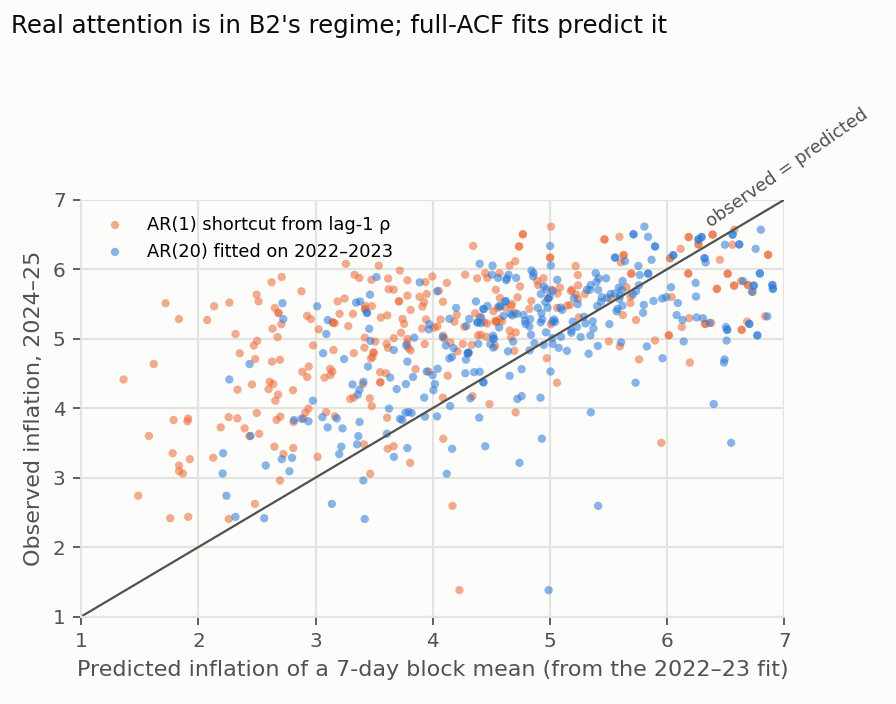
\includegraphics[width=0.62\linewidth]{../figures/r4_inflation.png}
\caption{Observed inflation of 7-day block means against the prediction from each article's prefix fit: the lag-1 shortcut (orange) and the full ACF of an AR(20) fit (blue).}\label{fig:inflation}
\end{figure}

\paragraph{Certified pooling on real-calibrated worlds.} We simulated 730-day worlds from AR(7) dynamics and an innovation covariance fitted to 30 Wikipedia articles (5 per community, community as the pooling component; sum of AR coefficients 0.92, weekly lag 0.18), with real residual vectors resampled independently over time, Gaussian shocks, or weekly residual blocks as a stress test. The learner observes a slate of 5 or 10 articles a day. We extended the innovation regression to AR($p$) through an augmented Kalman filter (verified to match the AR(1) implementation exactly).

\begin{figure}[t]\centering
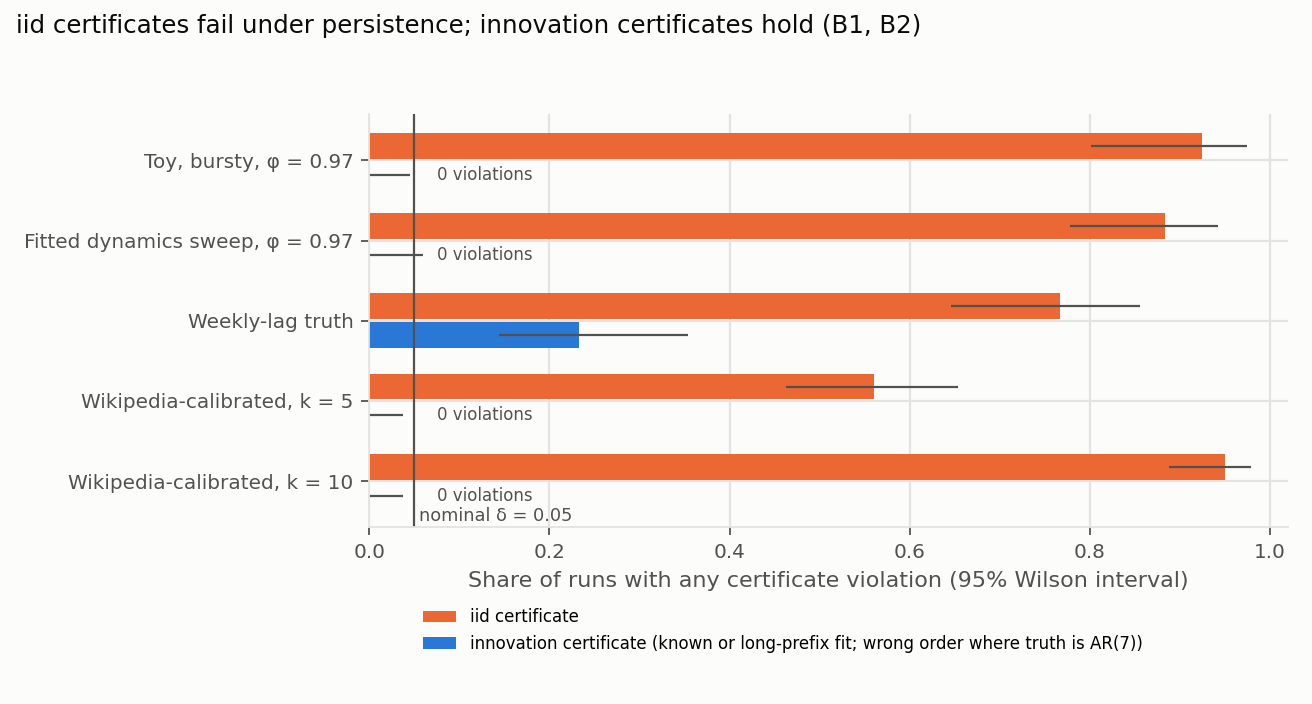
\includegraphics[width=0.9\linewidth]{../figures/r3_validity.png}
\caption{Share of runs with any certificate violation (95\% Wilson intervals) in the toy, the estimated-dynamics sweep, the weekly-lag misspecification, and worlds calibrated to Wikipedia attention.}\label{fig:validity}
\end{figure}

\begin{itemize}
\item \emph{iid certificates fail on real dynamics}: violated in 56\% (slate of 5) and 95\% (slate of 10) of runs, and 78--99\% under elimination.
\item \emph{Innovation certificates hold}: 0--1\% violations with known, re-fitted AR(7) and even AR(1)-fitted dynamics.
\item \emph{But they are too wide to act}: valid elimination eliminates nothing in 730 days and valid SP-UCB has about ten times the regret of the iid rule (455--466 against 37--47). The iid rule never dropped the best article here, because it leads by 0.135, a gap the iid rule's under-coverage did not cross.
\end{itemize}

\begin{figure}[t]\centering
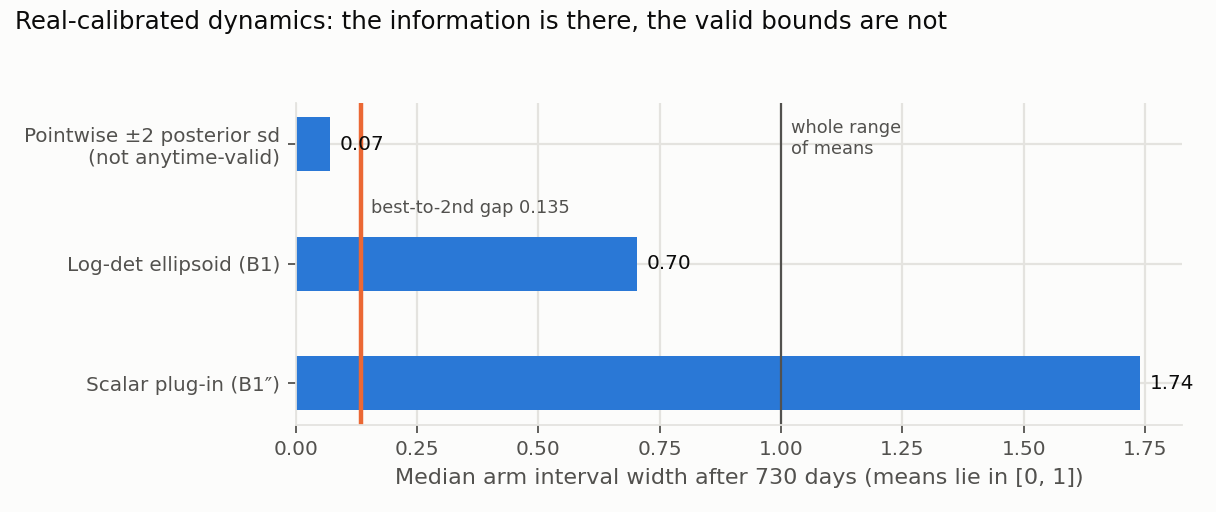
\includegraphics[width=0.85\linewidth]{../figures/r5_widths.png}
\caption{Median arm interval width after 730 days of 5-article slates on Wikipedia-calibrated dynamics, with the true model. The posterior is informative (pointwise width 0.07 against a 0.135 gap); the anytime-valid constructions are not.}\label{fig:widths}
\end{figure}

Figure~\ref{fig:widths} locates the problem. After two years the posterior standard deviation of each mean is 0.018 (pointwise $\pm2$ sd width 0.07), well inside the best-to-second gap. The log-determinant ellipsoid inflates it by $\beta\approx20$ (width 0.70) and the B1$''$ plug-in, whose cross-arm nuisance terms couple all 30 correlated arms, reaches 1.74, wider than the range of means. This is a statement about the certificate constructions, not about B1's theorem: the gap is a per-contrast anytime bound that pays $\sqrt{\log\log n}$ rather than $\sqrt{N\log T}$ after whitening the shocks.

\subsection{The slate contrast, exactly}

Proposition~\ref{prop:b3}(2) can be checked exactly from the covariance of the observed coordinates (Table~\ref{tab:slate}; Monte Carlo agrees within 0.3\%). The factor $1-\rho$ is exact for equal pairs; unequal variances or persistence give smaller gains, which the general long-run form predicts exactly. Under persistence the gain does not require simultaneous observation: alternating (staggered) observations keep 96--99\% of it, whereas under iid rewards they keep none.

\begin{table}[t]\centering\small
\begin{tabular}{lcccc}
\toprule
Pair ($n=365$ observations each) & $\rho=0.3$ & $\rho=0.6$ & $\rho=0.9$ & Staggered, $\rho=0.9$ \\
\midrule
Equal, $\varphi=0.9$ & 0.70 & 0.40 & 0.10 & 0.11 \\
Unequal sd (1 and 2) & 0.76 & 0.52 & 0.28 & 0.28 \\
$\varphi=0.9$ with $\varphi=0.5$ & 0.79 & 0.59 & 0.38 & 0.41 \\
Equal, iid & 0.70 & 0.41 & 0.11 & 1.00 \\
\bottomrule
\end{tabular}
\caption{Variance of a two-arm contrast relative to $\rho=0$.}\label{tab:slate}
\end{table}

\answer{Persistence must enter confidence sets. Under bursty exposure iid certificates are violated most of the time, by the amount B2 predicts, real Web attention is in that regime, and irrevocable decisions built on iid certificates drop the best arm. Innovation-regression certificates stay valid, including with dynamics estimated from a long prefix with the right lags. At Web persistence, however, today's anytime-valid constructions are 10--25 times wider than the information allows, so valid certificates rarely act; tightening them is the main open problem.}

%=====================================================================
\section{Q4. How should a learner act on persistent fluctuations?}\label{sec:q4}
%=====================================================================

\subsection{What theory says}

\paragraph{Joint filter.} Stacking long-run means and AR lags gives one Gaussian state that every observation updates for every arm and lag \src{S}. We verify the implementation against dense conditioning on the full node-time covariance.

\begin{proposition}[Innovation lower bound \src{S,P}]\label{prop:floor}
With stationary covariance $K_0$ and innovation covariance $Q_G$, every causal policy has dynamic regret at least $T\{\mathcal G(\mu,K_0)-\mathcal G(\mu,K_0-Q_G)\}$, $\mathcal G(\mu,K)=\E\max_i(\mu_i+Z_i)$.
\end{proposition}

\paragraph{Which uncertainty to explore.} Current-state Thompson sampling draws the fresh innovation, which no future observation will reveal; exploring it is pure cost. Predictive sampling \src{P} draws only the part that next round's rewards would reveal, $B=CV^{-1}C^\top$ with $C=\Cov(f_t,f_{t+1})$, $V=\Var(f_{t+1})$. Exploration of any kind pays only if enough future observations remain to use what it learns.

\begin{prediction}\label{pred:q4}
(a) Persistence-aware policies beat iid policies on persistent data. (b) Current-state Thompson sampling underperforms policies that explore persistent uncertainty. (c) Predictive exploration beats greedy use of the model only when each arm receives enough future observations. (d) A graph-shrunk shock covariance improves decisions only where shocks are correlated beyond a common factor and fluctuations decide the ranking.
\end{prediction}

\subsection{Evidence: a controlled benchmark}

\paragraph{Design.} 100 arms on a $10\times10$ grid; AR(20) coefficients proportional to $e^{-r/6}$ summing to 0.97; shocks correlated along the grid ($(I+5L)^{-1}$, unit diagonal); smooth long-run means; observation sd 0.3; $T=2{,}000$; 8 seeds; variants with weak persistence (0.6) and with independent shocks. Model-based policies know the dynamics; means are unknown.

\begin{figure}[t]\centering
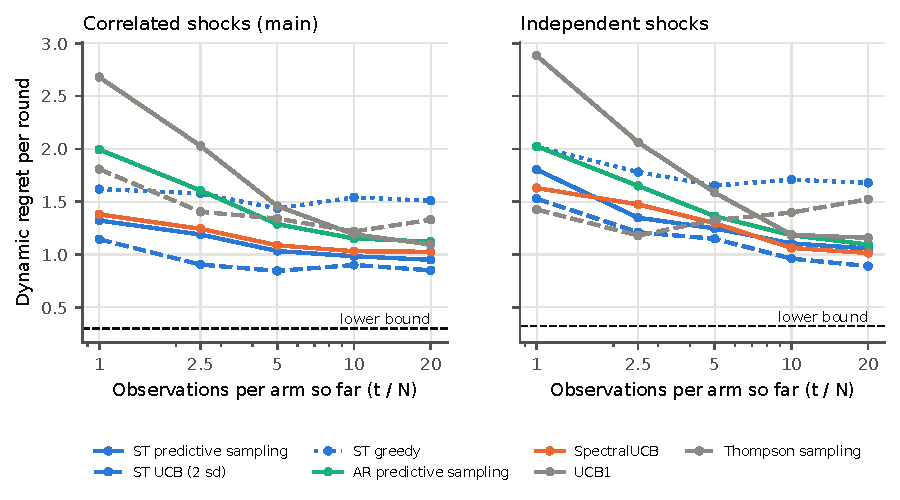
\includegraphics[width=\linewidth]{../figures/f4_toy_curves.pdf}
\caption{Benchmark: average dynamic regret over the first $t$ rounds (main configuration, left; independent shocks, right). Dashed: innovation lower bound.}\label{fig:toy}
\end{figure}

\begin{table}[t]\centering\small
\begin{tabular}{llccc}
\toprule
Policy & Models & Main & Independent shocks & Weak persistence \\
\midrule
ST UCB, 2 sd (tuned) & both channels & \textbf{0.850} & \textbf{0.890} & 1.856 \\
ST predictive sampling & both channels & 0.950 & 1.057 & 1.568 \\
SpectralUCB & mean channel only & 1.026 & 1.014 & 1.953 \\
UCB1 & nothing & 1.095 & 1.157 & 1.867 \\
AR predictive sampling & persistence only & 1.121 & 1.094 & \textbf{1.525} \\
ST current-state TS & both channels & 1.258 & 1.452 & 2.246 \\
Thompson sampling & nothing & 1.329 & 1.523 & 1.675 \\
ST greedy & both channels & 1.509 & 1.678 & 1.932 \\
\midrule
Innovation lower bound & & 0.298 & 0.323 & 1.276 \\
\bottomrule
\end{tabular}
\caption{Benchmark: dynamic regret per round at $T=2{,}000$.}\label{tab:toy}
\end{table}

\paragraph{Findings.} Joint predictive sampling, which has no tuning parameter, cuts dynamic regret 29\% against Thompson sampling and 13\% against UCB1, closing 37\% of the gap to the lower bound (tuned UCB closes 46\%; its multiplier was chosen on the same runs). Mis-targeted exploration is as harmful as having no model: greedy, current-state Thompson sampling (5\% better than TS) and the theory-constant UCB all lose to UCB1 (Prediction~\ref{pred:q4}b). Correlated shocks add 15\% on top of persistence (joint against persistence-only predictive sampling); with independent shocks the gain disappears (Prediction~\ref{pred:q4}d). Here fluctuations dominate the decision: their standard deviation (1.0) is twice the spread of long-run means (0.5).

\subsection{Evidence: KuaiRec under a chronological protocol}

\paragraph{Design.} Revision 2's daily panel built its co-engagement graph from the full log (79\% of its input rows postdate the first cutoff) and kept only videos observed on all 63 days. Revision 3 re-runs it chronologically. At each cutoff the graph is rebuilt from interactions dated before the first test day; eligible videos had at least 10 plays on every fit day, known at the cutoff; a video chosen on a day without plays returns nothing (availability is not known in advance). Three disjoint 11-day test windows (days 31--41, 42--52, 53--63), each fitted on all earlier days, times five predefined panels of 49--50 videos stratified by prefix popularity and community: 15 units. Budgets of 1 and 5 videos per day. Every hyperparameter (EWMA half-life, discount, window, UCB multiplier) is tuned on a development window (days 20--30, fit on 1--19) and frozen. Reward: logit of the daily complete-play rate. Intervals: bootstrap over windows, then panels.

\begin{table}[t]\centering\small
\begin{tabular}{lcc}
\toprule
Policy (regret relative to iid Thompson sampling) & $k=1$ & $k=5$ \\
\midrule
Joint filter, greedy & \textbf{0.47} [0.25, 0.70] & 0.44 [0.35, 0.52] \\
EWMA (tuned half-life) & 0.49 & 0.73 \\
Last observed value & 0.49 [0.28, 0.74] & \textbf{0.43} [0.31, 0.55] \\
Temporal-only filter, greedy & 0.50 & 0.46 \\
Joint filter, UCB & 0.51 [0.30, 0.73] & 0.46 [0.38, 0.54] \\
\quad same, rewired prefix graph / common factor only & 0.50 / 0.50 & 0.47 / 0.48 \\
Temporal-only filter, UCB & 0.51 & 0.52 \\
Sliding-window UCB & 0.61 & 0.74 \\
Discounted Thompson sampling & 0.77 & 0.90 \\
Seasonal naive (same weekday) & 1.00 & 1.01 \\
Static (fit-window mean) & 1.01 & 1.06 \\
\bottomrule
\end{tabular}
\caption{KuaiRec daily slot under the chronological protocol, regret per slot per day relative to iid Thompson sampling, 15 panel-window units.}\label{tab:chrono}
\end{table}

\paragraph{Findings.}
\begin{itemize}
\item \emph{Persistence pays, and the fix makes it larger} (Prediction~\ref{pred:q4}a). The joint filter cuts regret 49\% ($k=1$) and 54\% ($k=5$) against iid Thompson sampling, both intervals excluding zero; revision 2 reported 24--44\% on the retrospective panel.
\item \emph{The simplest persistence rule captures the gain.} Against the last observed value, the joint filter is $+3\%$ ($k=1$, interval $-13\%$ to $+43\%$) and $+7\%$ ($k=5$, $-10\%$ to $+61\%$): inconclusive. EWMA ties the filter at $k=1$; at $k=5$ its development-tuned half-life (7 days) generalized poorly, while its zero-half-life limit, the last value, matches the filter. Standard non-stationary bandits (discounted Thompson sampling, sliding-window UCB) are clearly worse than the filter.
\item \emph{Correlated shocks help when several items are compared each day} (Prediction~\ref{pred:q4}d, Proposition~\ref{prop:b3}(2)). At $k=5$ the shock covariance cuts regret 11\% against the temporal-only filter [5\%, 20\%]; at $k=1$ it does nothing ($-1\%$, $-6\%$ to $+4\%$). Most of the gain comes from a common factor: the prefix graph is indistinguishable from its rewiring ($-1.4\%$, $-6.6\%$ to $+3.5\%$) and from a common factor alone ($-3.5\%$, $-6.8\%$ to $+1.0\%$).
\item With strong priors from full fit-window logs and about one observation per video per window, greedy use of the model is at least as good as UCB.
\end{itemize}

\subsection{Evidence: Wikipedia and the Open Bandit Dataset}

\paragraph{Wikipedia (retrospective panels).} On log daily views of 150 articles with ten featured slots per day, models fitted on a rolling 365-day window and tested on the next 120 days at three origins, the drifting-level filter cuts regret 32\% against iid Thompson sampling on the one-domain panel ($-23\%$ against the last value), and the best model cuts it 24\% on the six-domain panel ($-16\%$ against the last value), where mild optimism (UCB, 1 sd) beats greedy by 9\%. On six domains, where hyperlinks carry community shocks, putting them into the shock covariance changes regret by $-2.0\%$ ($\pm1.3\%$) under predictive sampling and $+2.2\%$ ($\pm1.1\%$) under greedy: which articles lead is set mostly by long-run levels (fluctuation sd 0.48 against level spread 0.91). These panels were selected with later data and use a 2026 link snapshot. An independent chronological study on two other Wikipedia panels (dated graphs, a full year of 2025 test days) found the result panel-dependent: at one reading per day, static ranking and iid Thompson sampling are strongest; at five, the joint filter is 25\% below iid Thompson sampling on one panel but within 2.6\% of EWMA, and a temporal-only rule is best on the other.

\paragraph{Open Bandit Dataset.} Item click rates vary from day to day more than binomial noise allows (Pearson dispersion about 2 against a null 95th percentile of 1.3--1.4), but the excess does not persist: lag-1 autocorrelation of daily residuals is $-0.14$ to $-0.22$ and about 0 for six-hour bins, at 1--2 clicks per item per bin. There is no fluctuation channel to exploit, and an independent censored-learner pilot is underpowered (10--16 test clicks per trajectory). Prediction~\ref{pred:q4}a has nothing to act on here, which is itself consistent with it.

\begin{figure}[t]\centering
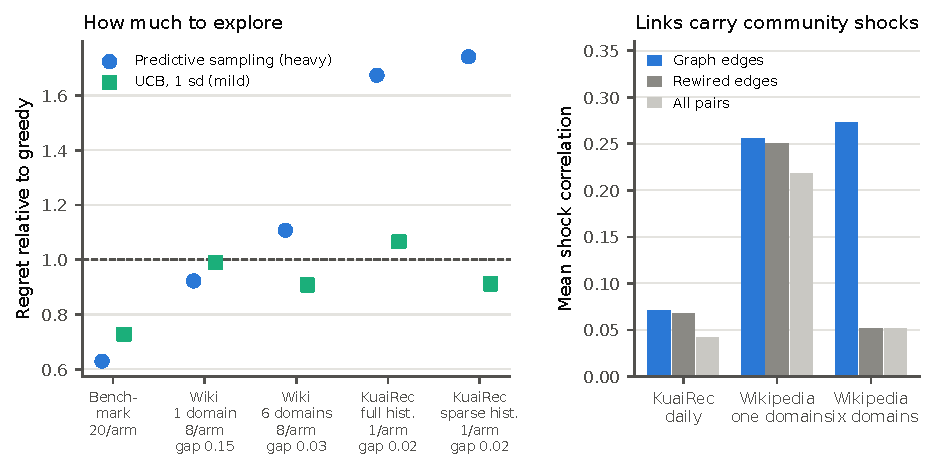
\includegraphics[width=\linewidth]{../figures/f5_synthesis.pdf}
\caption{Left: predictive sampling relative to greedy use of the same model, against the number of future observations each arm receives. Right: value of the graph in the shock covariance (held-out log-likelihood gain over a common-factor model) on the three daily panels. KuaiRec points use the retrospective panel.}\label{fig:synth}
\end{figure}

\subsection{Synthesis: when does exploration pay, and when does the model?}

\begin{table}[t]\centering\small
\resizebox{\linewidth}{!}{%
\begin{tabular}{lccccccc}
\toprule
Environment & Future obs. per arm & 10th--11th gap & Daily top-10 turnover & Fluctuation / level sd & Pred. sampling / greedy & UCB 1 sd / greedy & Best model / iid TS \\
\midrule
Benchmark & 20 & -- & -- & 2.0 & \textbf{0.63} & 0.73 & 0.71 \\
Wikipedia, one domain$^*$ & 8 & 0.15 & 3\% & 0.39 & \textbf{0.92} & 0.99 & 0.74 \\
Wikipedia, six domains$^*$ & 8 & 0.03 & 22\% & 0.52 & 1.11 & \textbf{0.91} & 0.76 \\
KuaiRec daily, full history$^*$ & 1.1 & 0.02 & 33\% & 0.85 & 1.67 & 1.07 & 0.62 \\
KuaiRec daily, sparse history$^*$ & 1.1 & 0.02 & 33\% & 0.85 & 1.74 & \textbf{0.91} & 0.56 \\
KuaiRec daily, chronological ($k=5$) & about 1 & -- & -- & -- & -- & 1.04$^\ddagger$ & 0.44 \\
\bottomrule
\end{tabular}}
\caption{When exploration pays. Ratios below 1 favour the exploring policy over greedy use of the same model. $^*$Retrospective panels. $^\ddagger$UCB with the development-tuned bonus (0.5 sd).}\label{tab:synth}
\end{table}

\paragraph{What the synthesis shows.}
\begin{itemize}
\item \emph{Persistence pays everywhere rewards persist}: persistence-aware policies have 24--56\% less regret than iid Thompson sampling. Whether a full model beats simple persistence rules depends on the setting: it does in the benchmark and on the retrospective Wikipedia panels, but not on the chronological KuaiRec panel.
\item \emph{How much to explore depends on observations per arm and on gaps} (Prediction~\ref{pred:q4}c). Heavy exploration of persistent uncertainty (predictive sampling) beats greedy only where arms receive many observations and the top is well separated or dominated by fluctuations. Mild optimism helps where priors are weak or rankings move; with strong priors and about one observation per arm, greedy is best.
\item \emph{The graph helps the fluctuation channel in proportion to how much shared shocks decide the ranking}: 15\% in the benchmark; 11\% at five items a day on chronological KuaiRec, through a common factor; at most $\pm3\%$ on six-domain Wikipedia, where levels decide the top ten.
\end{itemize}

\answer{Account for persistence: it is the largest real-data gain (about half of iid Thompson sampling's regret on a chronologically valid panel). On real panels a simple persistence rule (the last observed value) captures most of it, so the case for a full joint model rests on its uncertainty (certificates, exploration targeting), not its point forecasts. Explore only uncertainty that persists, matched to observations per arm. Put shared shocks into the model when several items are compared at once; a common factor captures most of their value.}

%=====================================================================
\section{Lessons, limitations and open problems}\label{sec:changes}
%=====================================================================

\paragraph{Claims revised since revision 2.}
\begin{itemize}
\item ``Modelling dynamics cuts regret by 24--43\%'' becomes ``persistence-aware policies halve regret; the last observed value captures most of it'' (chronological KuaiRec).
\item ``Certified gains track rejectability (median 0.84 $\to$ 0.40)'' is confirmed across certificates and on a second platform, but the per-instance link is weak at 360 instances.
\item ``Graphs help on average through shrinkage'' is sharpened: real graphs beat rewired nulls only under certification.
\item ``Innovation certificates are never violated, at comparable regret'' becomes ``valid, including with long-prefix estimated dynamics, but too wide to act at Web persistence''.
\item ``Hyperlinks change decisions by at most 3\%'' is retained but flagged as retrospective.
\item B3(2) is restated with the general long-run contrast formula; the $(1-\rho)$ factor needs equal variances.
\end{itemize}

\paragraph{A checklist for practitioners.}
\begin{enumerate}
\item \emph{Measure before trusting.} Compare each candidate graph with its rewiring on held-out data.
\item \emph{Certify pooling.} Uncertified pooling wins on average and fails selectively. Expect certified gains in proportion to the components the certificate can reject, and benchmark against graph-free empirical-Bayes shrinkage.
\item \emph{Account for persistence in every confidence statement,} especially when exposure is bursty, and fit the full lag structure (weekly lags on Web data).
\item \emph{Use persistence first.} The last observed value or a joint filter; standard discounting is not enough. Explore only persistent uncertainty, matched to observations per arm.
\item \emph{Check what decides the ranking.} If long-run levels dominate fluctuations, a graph in the shock model will barely change decisions.
\end{enumerate}

\paragraph{Limitations.} KuaiRec and Open Bandit Dataset ground truths are estimated (one watch ratio per user--video pair; four days of click rates), so mean-channel results are model-based evidence on real parameters, not logged-feedback evidence. Panel experiments assume showing an item does not change its organic demand (a monitoring setting). Our Wikipedia panels are retrospective; the KuaiRec log has no records for 11--26 August 2020, so later prefix graphs are stale. Replication units are modest (120 users; 15 panel-window units; 20 seeds per fixed instance), and seeds are not independent Web histories. Certified methods use fixed-level KL bounds, so all certified comparisons are within that family.

\paragraph{Open problems.} (1) \emph{A tighter anytime-valid certificate under correlated persistent shocks}: the information exists (pointwise width 0.07 against a 0.135 gap after two years) but current constructions are 10--25 times wider. (2) A valid and narrow mean-channel certificate on real graphs; level-matched calibration closes about half of the gap to the oracle. (3) Learning dynamics, including lag order, online while keeping certificates valid. (4) A chronological re-run of the six-community hyperlink result. (5) Geometry results (paths against cliques, graph error) on real graphs.

\appendix

%=====================================================================
\section{Proofs of the bridging results}\label{app:proofs}
%=====================================================================

\paragraph{B1 (Theorem~\ref{thm:b1}).} Define $U_i=\hat\mu_i+\beta_t\|e_i\|_{J_t^{-1}}$ and $U_c=\min\{\max_{i\in C_c}U_i,\min_{w\in\Delta(C_c)}(w^\top\hat\mu+\beta_t\|w\|_{J_t^{-1}})+\varepsilon_c\}$. \emph{Validity:} Theorem~\ref{thm:innov} holds for all contrasts simultaneously, hence for every $e_i$ and every $w$ in every simplex; for $w\in\Delta(C_c)$, $w^\top\mu\ge v_c-\varepsilon_c$, so both terms of $U_c$ bound $v_c=\max_{i\in C_c}\mu_i$. Minimizing over $w$ is free because the event does not depend on $w$. \emph{Regret:} if $c$ is selected at round $t$, then $\mu^\star\le U_c\le v_c+\varepsilon_c+2\beta_t\|w\|_{J_t^{-1}}$, so $\min_w\|w\|^2_{J_t^{-1}}\ge(\Gamma_c-\varepsilon_c)^2/(4\beta_t^2)$; the information-growth condition makes this at most $1/(\iota_c(N_c-1))$. Arms are identical, and summation follows Theorem~\ref{thm:spucb}. \emph{AR(1) constant:} with independent arms the information is diagonal. The coefficient of $\mu_i$ in a pull of arm $i$ is $1-\varphi^hs$, where $h\ge1$ is the gap since the arm's last observation and $s\in[0,1]$ is the filter's estimate after unit residuals, so it is at least $1-\varphi$; the predictive variance is at most $V+r$.

\paragraph{B1$'$ (Proposition~\ref{prop:b1p}).} With $Q_G$ diagonal and $H=\alpha I$, each $u_t$ has one nonzero entry, so each arm's score $W_i=\sum_{t:a_t=i}u_t\epsilon_t$ is a scalar martingale with quadratic variation $\I_{ii}$. The one-dimensional method of mixtures gives $|W_i|\le\sqrt{2J_{ii}\log(\sqrt{J_{ii}/\alpha}/\delta')}$ at all times with probability at least $1-\delta'$; the regularization bias is at most $\sqrt\alpha$. The pooled statistic $q_c/J_c$ with $J_c=\alpha+\sum_{i\in C_c}\I_{ii}$ estimates the information-weighted average of the pulled arms' means, which is at least $v_c-\varepsilon_c$, with a scalar martingale error. A union bound over $N+M$ statistics with $\delta'=\delta/(N+M)$ completes the proof.

\paragraph{B1$''$ (Proposition~\ref{prop:b1pp}).} Let $G=J-\alpha I$. Then $q_i-\sum_{j\ne i}G_{ij}m_j=G_{ii}\mu_i+\sum_{j\ne i}G_{ij}(\mu_j-m_j)+W_i$, where $W_i=\sum_tu_{t,i}\epsilon_t$ is a scalar martingale with quadratic variation $G_{ii}$. On the event $E$ that all scalar mixture bounds hold, and given intervals $[l_j,h_j]\ni\mu_j$ with midpoints $m_j$ and half-widths $\rho_j$, the error of $\hat\mu_i=(q_i-\sum_{j\ne i}G_{ij}m_j)/J_{ii}$ is at most $(\sqrt{2J_{ii}\log(\sqrt{J_{ii}/\alpha}/\delta')}+\alpha+\sum_{j\ne i}|G_{ij}|\rho_j)/J_{ii}$. Starting from $[0,1]$, induction keeps every interval true-containing on $E$. For components, write $\mu_i=\theta_c+d_i$ with $\theta_c$ the midrange and $|d_i|\le\varepsilon_c/2$; the design $P^\top u_t$ ($P$ the membership matrix) gives the same argument for $\theta$, with a deterministic deviation term $\sum_i|(P^\top G)_{ci}|\varepsilon_{c(i)}/2$, so $\hat\theta_c+\rho_c+\varepsilon_c/2\ge v_c$. With independent shocks $G$ is diagonal and the structure of SP-UCB is recovered. The cross terms $\sum_{j\ne i}|G_{ij}|\rho_j$ are what make the bound wide when many arms share correlated shocks (Figure~\ref{fig:widths}).

\paragraph{B1 for AR($p$).} Stack the lags into $s_t=(z_t,\dots,z_{t-p+1})$ with companion transition $A$ and innovation covariance $Q_G$ on the first block. The augmented filter tracks $s_t\mid\mathcal H_t\sim N(g_t+D_t\mu,P_t)$; observing arm $a$ gives the design vector $u=e_a+D_{a\cdot}$ and residual $y-g_a$ with variance $P_{aa}+r$, and updates $(g,D,P)$ by the Kalman gain $P_{\cdot a}/(P_{aa}+r)$ before propagating with $A$. Theorem~\ref{thm:innov} applies unchanged. With $p=1$ this reproduces the AR(1) recursion exactly, as verified numerically.

\paragraph{B2 (Proposition~\ref{prop:b2}).} Within a block of $b$ consecutive pulls the autocovariances are $V\varphi^{|s-u|}$; summing gives $\Var(\sum)=V[b\frac{1+\varphi}{1-\varphi}-\frac{2\varphi(1-\varphi^b)}{(1-\varphi)^2}]$. Blocks separated by other arms' blocks are nearly independent, so $n$ pulls in blocks have variance $(V/n)f(b,\varphi)$. For a general stationary process the same sum gives $f(b)=1+2\sum_{h<b}(1-h/b)\rho(h)$. The sample mean is Gaussian, giving the stated miscoverage.

\paragraph{B3 (Proposition~\ref{prop:b3}).} Part (1): after the initial lags, the full-field innovation transform $X_t-\sum_k\mathrm{diag}(a_k)X_{t-k}=D_c\mu+\eta_t$ adds information $D_cQ_G^{-1}D_c$ per field \src{S}; substituting this information for the count-based information in the change-of-measure program of \src{A} replaces $\sigma^2$ by $q/c^2$. Part (2): the sum of $n$ observations of arm $i$ minus that of arm $j$ has variance $\sum_{s,u}[\gamma_{ii}(s-u)+\gamma_{jj}(s-u)-2\gamma_{ij}(s-u)]$, which divided by $n^2$ converges to $(\Omega_{ii}+\Omega_{jj}-2\Omega_{ij})/n$ with $\Omega=\sum_h\gamma(h)$; with equal variances and common dynamics $\Omega_{ij}=\rho\,\Omega_{ii}$. For staggered observations the cross-covariances at lag one replace those at lag zero; under persistence they are nearly equal, under iid rewards they vanish.

%=====================================================================
\section{Data and graph construction}\label{app:data}
%=====================================================================

\paragraph{KuaiRec.} Small matrix: 1,411 users $\times$ 3,327 videos, 4,676,570 interactions. Big matrix: 7,176 $\times$ 10,728, 12,530,806 interactions, no overlap with the small matrix, no records dated 11--26 August 2020. Reward R1 $=\min(\text{watch ratio},5)/5$. Graphs are union-$k$NN with Laplacians scaled to mean degree one; nulls are degree-preserving rewirings. U-coeng: Jaccard on fully watched non-evaluation videos. U-mf and I-mf: PureSVD (rank 64) on leakage-free splits. I-coeng: IDF-weighted engagement from non-evaluation users; in the chronological daily experiment it is rebuilt at each cutoff from rows dated before the first test day. Other graphs as in revision 2.

\paragraph{Wikipedia.} Public Wikimedia REST API (daily user page views, 2022--2025) and MediaWiki links API (2026 snapshot). One domain: 150 most-viewed programming-language articles with complete data. Six domains: 25 articles each from NFL teams, NBA teams, MLB teams, Premier League clubs, UN member states and programming languages; 84\% of 1,990 hyperlinks within a domain.

\paragraph{Open Bandit Dataset.} ZOZOTOWN, 24--30 November 2019, uniform-random logs (CC BY 4.0): All (1,374,327 impressions, 80 items, 4,768 clicks), Men (452,949; 34; 2,321), Women (864,585; 46; 4,163). Positions differ by under 10\% in click rate.

%=====================================================================
\section{Reproducibility}\label{app:repro}
%=====================================================================

Each experiment has its own directory under \texttt{experiments/} holding its design, code, results and report; \texttt{experiments/report} maps all of them to the theory. From the repository root:

{\footnotesize
\begin{verbatim}
# Q1-Q2 (KuaiRec): alignment, Settings A, A v2 (360 instances), B
python -I experiments/kuairec/code/{data,graphs,alignment,setting_a,setting_b}.py
python -I experiments/oct10_evening/code/setting_a2_expand.py
# Q2 (Open Bandit Dataset)
python -I experiments/oct10_runs/code/{obd_feasibility,obd_pooling}.py
# Q3: certificates under persistence, estimated dynamics, B2/B3 instances,
#     real inflation, Wikipedia-calibrated worlds
python -I experiments/simulations/certificates_under_persistence/code/coverage.py --tag _plugin
python -I experiments/oct10_runs/code/{robustness,theory_instances,inflation}.py
python -I experiments/oct10_evening/code/certificates_real.py
# Q4: benchmark, chronological KuaiRec daily, Wikipedia
python -I experiments/simulations/spatiotemporal_benchmark/code/toy.py [--extra]
python -I experiments/oct10_evening/code/daily_chrono.py
python -I experiments/wikipedia/code/attention.py [--dataset multi]
# cross-experiment analyses and figures
python -I experiments/report/code/build_report.py
\end{verbatim}}

\end{document}
